\documentclass[10pt]{beamer}
\usetheme{metropolis}
\usepackage{booktabs}
\usepackage{tabularx}
\usepackage{calc}
\usepackage{tikz}
\usetikzlibrary{shapes.geometric, arrows, positioning, decorations.pathreplacing, patterns}
\usepackage[sfdefault]{FiraSans}
\usepackage[scaled]{FiraMono}

% Setup for faculty images
\newlength{\imageheight}
\setlength{\imageheight}{3.5cm}

% Define CSUF brand colors
\definecolor{titanblue}{HTML}{00244E}
\definecolor{mediumblue}{HTML}{0F3F8C}
\definecolor{skyblue}{HTML}{EBFBFF}
\definecolor{titanorange}{HTML}{FF7900}
\definecolor{titangray}{HTML}{F5F5F5}
\definecolor{titantext}{HTML}{222222}

% Customize metropolis theme colors
\setbeamercolor{normal text}{fg=titantext, bg=white}
\setbeamercolor{alerted text}{fg=titanorange}
\setbeamercolor{example text}{fg=mediumblue}

% Title page colors
\setbeamercolor{title}{fg=titanblue, bg=white}
\setbeamercolor{subtitle}{fg=mediumblue, bg=white}
\setbeamercolor{institute}{fg=titanorange, bg=white}
\setbeamercolor{date}{fg=titanblue, bg=white}

% Frame title colors
\setbeamercolor{frametitle}{fg=white, bg=titanblue}
\setbeamercolor{framesubtitle}{fg=mediumblue, bg=white}

% Block environment colors
\setbeamercolor{block title}{fg=white, bg=titanblue}
\setbeamercolor{block body}{fg=titantext, bg=skyblue!10}

% Item colors
\setbeamercolor{itemize item}{fg=titanorange}
\setbeamercolor{itemize subitem}{fg=mediumblue}
\setbeamercolor{itemize subsubitem}{fg=titanblue}

% Footer and header colors
\setbeamercolor{footer}{fg=titantext}
\setbeamercolor{header}{fg=titanblue}

% Customize fonts
\setbeamerfont{title}{size=\Large, series=\bfseries}
\setbeamerfont{frametitle}{size=\large, series=\bfseries}

% Simple title page template
\defbeamertemplate*{title page}{customized}[1][]
{
\vspace{1cm}
 {\usebeamerfont{title}\usebeamercolor[fg]{title}\inserttitle\par}
\vspace{0.5cm}
 {\usebeamerfont{subtitle}\usebeamercolor[fg]{subtitle}\insertsubtitle\par}
\vspace{0.5cm}
 {\usebeamerfont{date}\usebeamercolor[fg]{date}\insertdate\par}
\vfill
 {\insertinstitute\par}
}

% Add progress bar - FIXED VERSION
\makeatletter
\setbeamertemplate{headline}{%
\begin{beamercolorbox}[wd=\paperwidth,ht=0.4cm,dp=0cm]{titanblue}%
\begin{tikzpicture}
\pgfmathsetmacro{\progress}{\insertframenumber/\inserttotalframenumber}
\fill[titanorange] (0,0) rectangle (\progress*\paperwidth,0.4cm);
\end{tikzpicture}%
\end{beamercolorbox}%
}
\makeatother

\begin{document}

\title{Understanding Politics and Public Policy}
\subtitle{Foundations and Core Concepts\\POSC 315: Introduction to Public Policy\\Lecture 8-2\\Decision Making (Part 2 of 3)}
\author{Dr. David P. Adams}
\date{Summer 2025}
\institute{California State University, Fullerton}

\maketitle

\begin{frame}{Where We Are}
\begin{center}
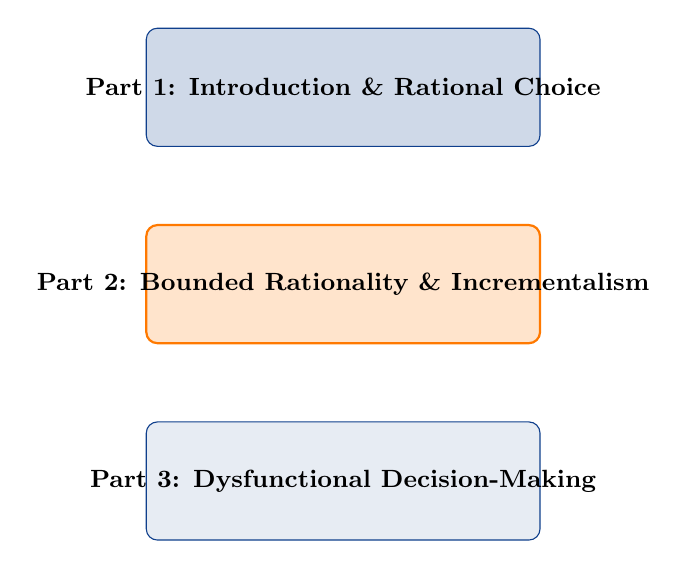
\begin{tikzpicture}[node distance=2cm]
% Better sized boxes to accommodate text
\node[rectangle, rounded corners, minimum width=5cm, minimum height=1.5cm, draw=mediumblue, fill=mediumblue!20] (part1) at (0,0) {};
\node[rectangle, rounded corners, minimum width=5cm, minimum height=1.5cm, draw=titanorange, fill=titanorange!20, thick] (part2) at (0,-2.5) {};
\node[rectangle, rounded corners, minimum width=5cm, minimum height=1.5cm, draw=mediumblue, fill=mediumblue!10] (part3) at (0,-5) {};

% Text positioned properly within boxes
\node[font=\small\bfseries] at (part1.center) {Part 1: Introduction \& Rational Choice};
\node[font=\small\bfseries] at (part2.center) {Part 2: Bounded Rationality \& Incrementalism};
\node[font=\small\bfseries] at (part3.center) {Part 3: Dysfunctional Decision-Making};
\end{tikzpicture}
\end{center}
\end{frame}

\begin{frame}{Recap: Rational Choice Theory}
\begin{center}
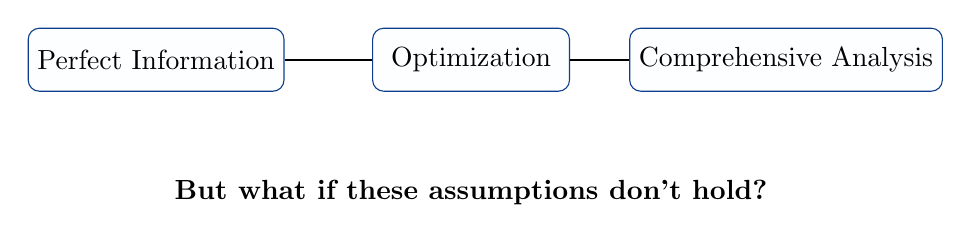
\begin{tikzpicture}[node distance=1.5cm]
\node[rectangle, rounded corners, minimum width=2.5cm, minimum height=0.8cm, draw=mediumblue, fill=skyblue!15] (perfect) at (0,0) {Perfect Information};
\node[rectangle, rounded corners, minimum width=2.5cm, minimum height=0.8cm, draw=mediumblue, fill=skyblue!15] (optimize) at (4,0) {Optimization};
\node[rectangle, rounded corners, minimum width=2.5cm, minimum height=0.8cm, draw=mediumblue, fill=skyblue!15] (comprehensive) at (8,0) {Comprehensive Analysis};

\draw[-, thick] (perfect) -- (optimize);
\draw[-, thick] (optimize) -- (comprehensive);

% Added missing semicolon here
\node[below=1cm of optimize] {\textbf{But what if these assumptions don't hold?}};
\end{tikzpicture}
\end{center}
\end{frame}

\begin{frame}{Bounded Rationality}
\begin{center}
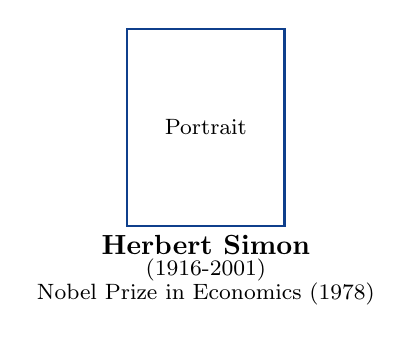
\begin{tikzpicture}
% Portrait placeholder
\draw[thick, mediumblue] (0,0) rectangle (2,2.5);
\node at (1,1.25) {\footnotesize Portrait};
\node[below] at (1,0) {\textbf{Herbert Simon}};
\node[below] at (1,-0.3) {\footnotesize (1916-2001)};
\node[below] at (1,-0.6) {\footnotesize Nobel Prize in Economics (1978)};
\end{tikzpicture}
\end{center}

\begin{block}{Key Quote}
``The capacity of the human mind for formulating and solving complex problems is very small compared with the size of the problems whose solution is required for objectively rational behavior in the real world.''
\end{block}
\end{frame}

\begin{frame}{Core Concepts in Bounded Rationality}
\begin{columns}
\begin{column}{0.5\textwidth}
\begin{block}{Intertwined Elements}
\begin{itemize}
\item Goals and tools are considered together
\item Means and ends are not separate
\item Values and facts are interconnected
\end{itemize}
\end{block}
\end{column}
\begin{column}{0.5\textwidth}
\begin{block}{Definition of ``Good'' Policy}
A ``good'' policy is one where \textcolor{titanorange}{\textbf{consensus can be reached}} among stakeholders.
\end{block}
\end{column}
\end{columns}
\end{frame}

\begin{frame}{The ``Administrative Man''}
Bounded rationality recognizes that human rationality is limited:

\vspace{0.5cm}
\begin{center}
\begin{tikzpicture}[node distance=1cm]
\node[circle, minimum size=1.5cm, draw=titanblue, fill=skyblue!20, thick, font=\footnotesize, align=center] (center) at (0,0) {\textbf{Bounded\\Rationality}};

\node[ellipse, minimum width=2.8cm, minimum height=0.8cm, draw=titanorange, fill=titanorange!10, font=\footnotesize, align=center] (info) at (-2.5,2) {Limited\\Information};
\node[ellipse, minimum width=2.8cm, minimum height=0.8cm, draw=titanorange, fill=titanorange!10, font=\footnotesize, align=center] (time) at (2.5,2) {Limited\\Time};
\node[ellipse, minimum width=2.8cm, minimum height=0.8cm, draw=titanorange, fill=titanorange!10, font=\footnotesize, align=center] (cognitive) at (-3,0) {Limited Cognitive\\Capacity};
\node[ellipse, minimum width=2.8cm, minimum height=0.8cm, draw=titanorange, fill=titanorange!10, font=\footnotesize, align=center] (resources) at (3,0) {Limited\\Resources};
\node[ellipse, minimum width=2.8cm, minimum height=0.8cm, draw=titanorange, fill=titanorange!10, font=\footnotesize, align=center] (processing) at (-2.5,-2) {Limited Information\\Processing};
\node[ellipse, minimum width=2.8cm, minimum height=0.8cm, draw=titanorange, fill=titanorange!10, font=\footnotesize, align=center] (priorities) at (2.5,-2) {Competing\\Priorities};

% Draw arrows - FIXED \foreach variable
\foreach \nodename in {info, time, cognitive, resources, processing, priorities} {
    \draw[-, thick] (\nodename) -- (center);
}
\end{tikzpicture}
\end{center}
\end{frame}

\begin{frame}{Satisficing in Bounded Rationality}
\begin{center}
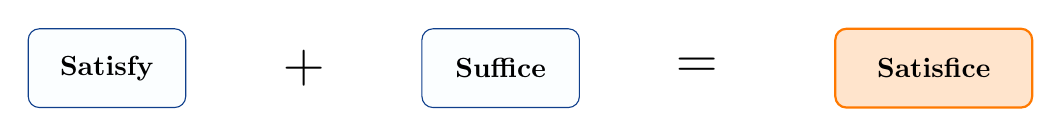
\begin{tikzpicture}[node distance=2cm]
% Create equation-like layout
\node[rectangle, rounded corners, minimum width=2cm, minimum height=1cm, draw=mediumblue, fill=skyblue!20] (satisfy) at (0,0) {\textbf{Satisfy}};
\node (plus) at (2.5,0) {\huge +};
\node[rectangle, rounded corners, minimum width=2cm, minimum height=1cm, draw=mediumblue, fill=skyblue!20] (suffice) at (5,0) {\textbf{Suffice}};
\node (equals) at (7.5,0) {\huge =};
\node[rectangle, rounded corners, minimum width=2.5cm, minimum height=1cm, draw=titanorange, fill=titanorange!20, thick] (satisfice) at (10.5,0) {\textbf{Satisfice}};
\end{tikzpicture}
\end{center}

\vspace{1cm}
\begin{block}{Key Principles}
\begin{itemize}
\item Administrative actors choose the first option that meets \textcolor{titanorange}{\textbf{minimum criteria}}
\item Makes the most rational decision with available information
\item Achieves satisfactory (not maximum) social gain
\item Recognizes that further search for solutions has costs
\end{itemize}
\end{block}
\end{frame}

\begin{frame}{Rational Choice vs. Bounded Rationality}
\begin{center}
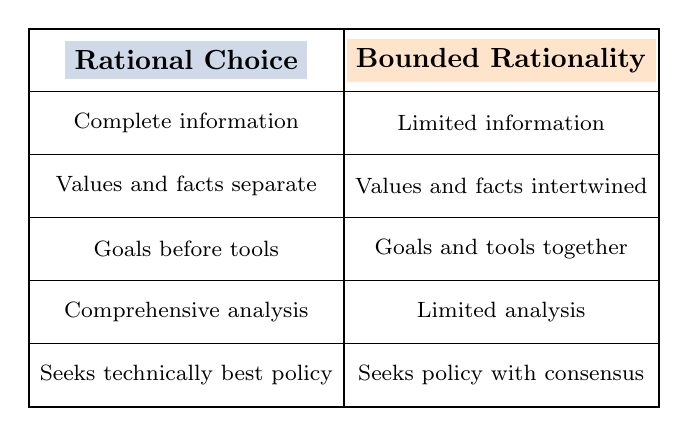
\begin{tikzpicture}[scale=0.8]
% Create comparison table
\draw[thick] (0,0) rectangle (10,6);

% Headers
\node[fill=mediumblue!20] at (2.5,5.5) {\textbf{Rational Choice}};
\node[fill=titanorange!20] at (7.5,5.5) {\textbf{Bounded Rationality}};

% Vertical divider
\draw[thick] (5,0) -- (5,6);

% Row dividers
\foreach \y in {1,2,3,4,5} {
    \draw (0,\y) -- (10,\y);
}

% Left column content
\node[align=center] at (2.5,4.5) {\footnotesize Complete information};
\node[align=center] at (2.5,3.5) {\footnotesize Values and facts separate};
\node[align=center] at (2.5,2.5) {\footnotesize Goals before tools};
\node[align=center] at (2.5,1.5) {\footnotesize Comprehensive analysis};
\node[align=center] at (2.5,0.5) {\footnotesize Seeks technically best policy};

% Right column content
\node[align=center] at (7.5,4.5) {\footnotesize Limited information};
\node[align=center] at (7.5,3.5) {\footnotesize Values and facts intertwined};
\node[align=center] at (7.5,2.5) {\footnotesize Goals and tools together};
\node[align=center] at (7.5,1.5) {\footnotesize Limited analysis};
\node[align=center] at (7.5,0.5) {\footnotesize Seeks policy with consensus};
\end{tikzpicture}
\end{center}
\end{frame}

\begin{frame}{Bounded Rationality: Example}
\begin{block}{Case: City Homelessness Response}
\end{block}

\begin{columns}
\begin{column}{0.5\textwidth}
\textbf{Decision Context}
\begin{itemize}
\item Rising homeless population
\item Mayor facing re-election in 6 months
\item Limited city budget
\item Incomplete data on homeless demographics
\item Multiple stakeholders with competing interests
\end{itemize}
\end{column}
<begin{column}{0.5\textwidth}
\textbf{Satisficing Approach}
\begin{itemize}
\item Review 3-4 policy options (not all possible alternatives)
\item Set minimum criteria: implementable within 4 months, cost under \$2M, address immediate shelter needs
\item Select first option that meets all criteria
\item Choose temporary shelter expansion despite knowing it's not the optimal solution
\end{itemize}
\end{column}
\end{columns}
\end{frame}

\begin{frame}{Incrementalism}
\begin{center}

\begin{tikzpicture}
% Portrait placeholder
\draw[thick, mediumblue] (0,0) rectangle (2,2.5);
\node at (1,1.25) {\footnotesize Portrait};
\node[below] at (1,0) {\textbf{Charles Lindblom}};
\node[below] at (1,-0.3) {\footnotesize (1917-2018)};
\node[below] at (1,-0.6) {\footnotesize ``The Science of Muddling Through'' (1959)};
\end{tikzpicture}
\end{center}

\vspace{0.5cm}
\begin{block}{Foundation}
Builds on Herbert Simon's work on bounded rationality
\begin{itemize}
\item Recognizes limited information processing capacity
\item Focuses on making small, manageable changes
\item Reduces risk through incremental adjustments
\end{itemize}
\end{block}
\end{frame}

\begin{frame}{Successive Limited Comparisons}
\begin{center}
\begin{tikzpicture}[node distance=2cm]
% Central status quo
\node[circle, minimum size=2cm, draw=titanblue, fill=skyblue!20, thick, font=\small, align=center] (sq) at (0,0) {\textbf{Status\\Quo}};

% Alternatives around it
\node[rectangle, rounded corners, minimum width=1.8cm, minimum height=0.8cm, draw=mediumblue, fill=mediumblue!10, font=\footnotesize] (alt1) at (0,2.5) {Alternative 1};
\node[rectangle, rounded corners, minimum width=1.8cm, minimum height=0.8cm, draw=mediumblue, fill=mediumblue!10, font=\footnotesize] (alt2) at (2,1.5) {Alternative 2};
\node[rectangle, rounded corners, minimum width=1.8cm, minimum height=0.8cm, draw=mediumblue, fill=mediumblue!10, font=\footnotesize] (alt3) at (2.5,0) {Alternative 3};
\node[rectangle, rounded corners, minimum width=1.8cm, minimum height=0.8cm, draw=mediumblue, fill=mediumblue!10, font=\footnotesize] (alt4) at (2,-1.5) {Alternative 4};
\node[rectangle, rounded corners, minimum width=1.8cm, minimum height=0.8cm, draw=mediumblue, fill=mediumblue!10, font=\footnotesize] (alt5) at (0,-2.5) {Alternative 5};
\node[rectangle, rounded corners, minimum width=1.8cm, minimum height=0.8cm, draw=mediumblue, fill=mediumblue!10, font=\footnotesize] (alt6) at (-2.5,0) {Alternative 6};

% Arrows showing small distances
\foreach \alt in {alt1, alt2, alt3, alt4, alt5, alt6} {
    \draw[-, thick, titanorange] (sq) -- (\alt);
}

% Highlight chosen alternative
\draw[titanorange, thick, dashed] (alt2.north west) rectangle (alt2.south east);
\end{tikzpicture}
\end{center}

\vspace{0.5cm}
\begin{itemize}
\item Compare alternatives to the \textcolor{titanorange}{\textbf{status quo}}
\item Choose the alternative that is the \textcolor{titanorange}{\textbf{least different}} from current policy
\end{itemize}
\end{frame}

\begin{frame}{Benefits of Incrementalism}
\begin{columns}
\begin{column}{0.5\textwidth}
\begin{block}{Simplifies Decision-Making}
\begin{itemize}
\item Reduces alternatives to consider
\item Focuses on marginal changes
\item Allows reliance on feedback
\end{itemize}
\end{block}
\end{column}
\begin{column}{0.5\textwidth}
\begin{block}{Manages Risk}
\begin{itemize}
\item Makes process serial and remedial
\item Avoids large, irreversible errors
\item Enables course correction
\end{itemize}
\end{block}
\end{column}
\end{columns}

\vspace{1cm}
\begin{center}
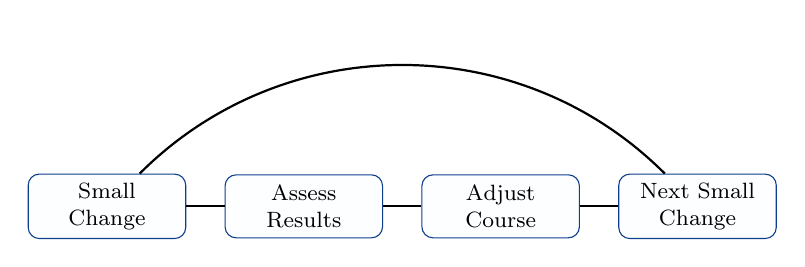
\begin{tikzpicture}[node distance=1.5cm]
\node[rectangle, rounded corners, minimum width=2cm, minimum height=0.8cm, draw=mediumblue, fill=skyblue!15, font=\footnotesize, align=center] (step1) at (0,0) {Small\\Change};
\node[rectangle, rounded corners, minimum width=2cm, minimum height=0.8cm, draw=mediumblue, fill=skyblue!15, font=\footnotesize, align=center] (step2) at (2.5,0) {Assess\\Results};
\node[rectangle, rounded corners, minimum width=2cm, minimum height=0.8cm, draw=mediumblue, fill=skyblue!15, font=\footnotesize, align=center] (step3) at (5,0) {Adjust\\Course};
\node[rectangle, rounded corners, minimum width=2cm, minimum height=0.8cm, draw=mediumblue, fill=skyblue!15, font=\footnotesize, align=center] (step4) at (7.5,0) {Next Small\\Change};

\draw[-, thick] (step1) -- (step2);
\draw[-, thick] (step2) -- (step3);
\draw[-, thick] (step3) -- (step4);
\draw[-, thick] (step4) to [bend right=45] (step1);
\end{tikzpicture}
\end{center}
\end{frame}

\begin{frame}{Limitations of Incrementalism}
\begin{block}{Not Always Appropriate}
\begin{itemize}
\item Some problems are too complex for incremental solutions
\item Some problems are too urgent to address incrementally
\item Some problems require fundamental, not incremental, change
\end{itemize}
\end{block}

\vspace{0.5cm}
\textbf{When ``Muddling Through'' Won't Work}

Some decisions require huge leaps:
\begin{itemize}
\item Moonshots \& major technological initiatives
\item Responses to wars \& national security threats
\item Managing pandemics \& public health emergencies
\item Addressing economic depressions \& major recessions
\end{itemize}
\end{frame}

\begin{frame}{Incrementalism: Example}
\begin{block}{Case: Environmental Regulation}
\end{block}

\begin{columns}
\begin{column}{0.5\textwidth}
\textbf{Status Quo}
\begin{itemize}
\item Current emissions standard: 30 parts per million
\item Industry has invested in existing compliance technology
\item Environmental groups want 10ppm standard
\item Economic concerns about rapid changes
\end{itemize}
\end{column}
<begin{column}{0.5\textwidth}
\begin{center}
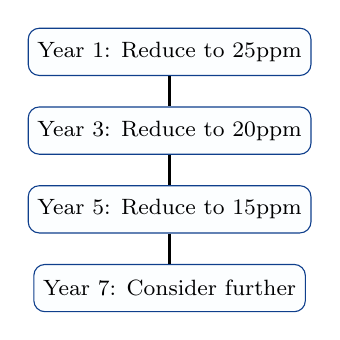
\begin{tikzpicture}[node distance=0.8cm]
\node[rectangle, rounded corners, minimum width=3cm, minimum height=0.6cm, draw=mediumblue, fill=skyblue!15, font=\footnotesize] (year1) at (0,0) {Year 1: Reduce to 25ppm};
\node[rectangle, rounded corners, minimum width=3cm, minimum height=0.6cm, draw=mediumblue, fill=skyblue!15, font=\footnotesize] (year3) at (0,-1) {Year 3: Reduce to 20ppm};
\node[rectangle, rounded corners, minimum width=3cm, minimum height=0.6cm, draw=mediumblue, fill=skyblue!15, font=\footnotesize] (year5) at (0,-2) {Year 5: Reduce to 15ppm};
\node[rectangle, rounded corners, minimum width=3cm, minimum height=0.6cm, draw=mediumblue, fill=skyblue!15, font=\footnotesize] (year7) at (0,-3) {Year 7: Consider further};

\draw[-, thick] (year1) -- (year3);
\draw[-, thick] (year3) -- (year5);
\draw[-, thick] (year5) -- (year7);
\end{tikzpicture}
\end{center}

\vspace{0.3cm}
\footnotesize{Each step builds on previous experience and allows for adjustment based on feedback and new information.}
\end{column}
\end{columns}
\end{frame}

\begin{frame}{Three Models Compared}
\begin{center}
\begin{tikzpicture}[node distance=3cm]
\node[rectangle, rounded corners, minimum width=2.5cm, minimum height=2cm, draw=titanblue, align=center, fill=mediumblue!10] (rational) at (0,0) {\textbf{Rational\\Choice}\\[0.3cm]\footnotesize Complete info\\Optimization\\Comprehensive};
\node[rectangle, rounded corners, minimum width=2.5cm, minimum height=2cm, draw=titanblue, align=center, fill=mediumblue!20] (bounded) at (4,0) {\textbf{Bounded\\Rationality}\\[0.3cm]\footnotesize Limited info\\Satisficing\\Consensus};
\node[rectangle, rounded corners, minimum width=2.5cm, minimum height=2cm, draw=titanblue, align=center, fill=mediumblue!30] (incremental) at (8,0) {\textbf{Incrementalism}\\[0.3cm]\footnotesize Small changes\\Status quo\\Serial process};

% Decision complexity arrow
\draw[very thick, titanorange] (0,-2) -- (8,-2);
\node[below] at (4,-2.5) {\footnotesize Increasing practical applicability};
\end{tikzpicture}
\end{center}
\end{frame}

\begin{frame}{When to Use Each Model}
\begin{center}
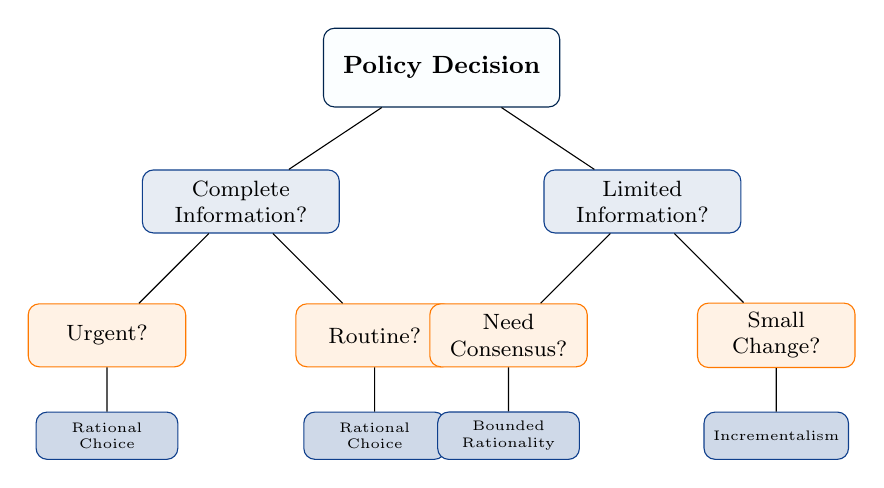
\begin{tikzpicture}[scale=0.85]
% Create decision tree
\node[rectangle, rounded corners, minimum width=3cm, minimum height=1cm, draw=titanblue, fill=skyblue!20, font=\small, align=center] (start) at (0,0) {\textbf{Policy Decision}};

% First branch - information availability
\node[rectangle, rounded corners, minimum width=2.5cm, minimum height=0.8cm, draw=mediumblue, fill=mediumblue!10, font=\footnotesize, align=center] (complete) at (-3,-2) {Complete\\Information?};
\node[rectangle, rounded corners, minimum width=2.5cm, minimum height=0.8cm, draw=mediumblue, fill=mediumblue!10, font=\footnotesize, align=center] (limited) at (3,-2) {Limited\\Information?};

% Second branch - urgency
\node[rectangle, rounded corners, minimum width=2cm, minimum height=0.8cm, draw=titanorange, fill=titanorange!10, font=\footnotesize] (urgent) at (-5,-4) {Urgent?};
\node[rectangle, rounded corners, minimum width=2cm, minimum height=0.8cm, draw=titanorange, fill=titanorange!10, font=\footnotesize] (routine) at (-1,-4) {Routine?};
\node[rectangle, rounded corners, minimum width=2cm, minimum height=0.8cm, draw=titanorange, fill=titanorange!10, font=\footnotesize, align=center] (consensus) at (1,-4) {Need\\Consensus?};
\node[rectangle, rounded corners, minimum width=2cm, minimum height=0.8cm, draw=titanorange, fill=titanorange!10, font=\footnotesize, align=center] (incremental) at (5,-4) {Small\\Change?};

% Final recommendations
\node[rectangle, rounded corners, minimum width=1.8cm, minimum height=0.6cm, draw=mediumblue, fill=mediumblue!20, font=\tiny, align=center] (rc1) at (-5,-5.5) {Rational\\Choice};
\node[rectangle, rounded corners, minimum width=1.8cm, minimum height=0.6cm, draw=mediumblue, fill=mediumblue!20, font=\tiny, align=center] (rc2) at (-1,-5.5) {Rational\\Choice};
\node[rectangle, rounded corners, minimum width=1.8cm, minimum height=0.6cm, draw=mediumblue, fill=mediumblue!20, font=\tiny, align=center] (br) at (1,-5.5) {Bounded\\Rationality};
\node[rectangle, rounded corners, minimum width=1.8cm, minimum height=0.6cm, draw=mediumblue, fill=mediumblue!20, font=\tiny, align=center] (inc) at (5,-5.5) {Incrementalism};

% Draw connections
\draw[-] (start) -- (complete);
\draw[-] (start) -- (limited);
\draw[-] (complete) -- (urgent);
\draw[-] (complete) -- (routine);
\draw[-] (limited) -- (consensus);
\draw[-] (limited) -- (incremental);
\draw[-] (urgent) -- (rc1);
\draw[-] (routine) -- (rc2);
\draw[-] (consensus) -- (br);
\draw[-] (incremental) -- (inc);
\end{tikzpicture}
\end{center}
\end{frame}

\begin{frame}{Key Takeaways: Alternative Models}
\begin{center}
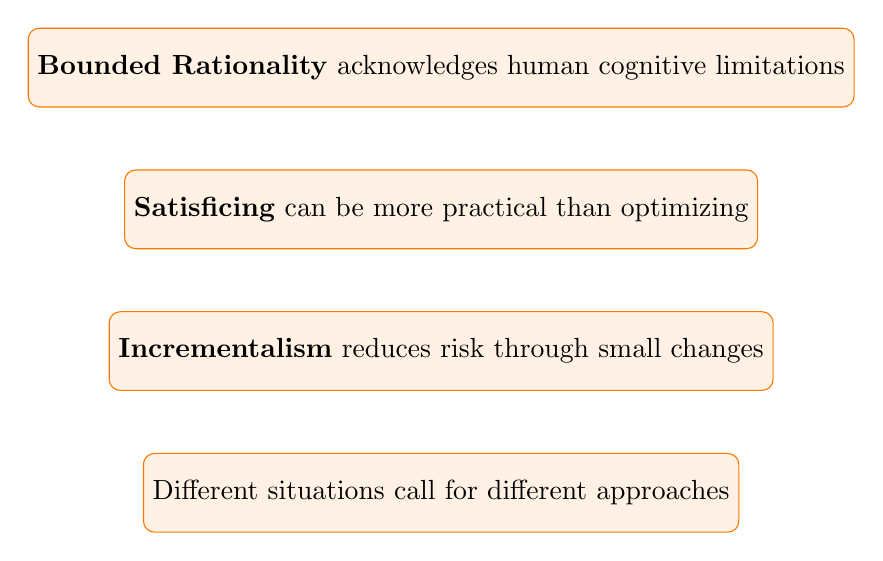
\begin{tikzpicture}[node distance=1.5cm]
% Added missing semicolons to all nodes
\node[rectangle, rounded corners, minimum width=7cm, minimum height=1cm, draw=titanorange, fill=titanorange!10, align=center] (t1) at (0,0) {\textbf{Bounded Rationality} acknowledges human cognitive limitations};
\node[rectangle, rounded corners, minimum width=7cm, minimum height=1cm, draw=titanorange, fill=titanorange!10, align=center] (t2) at (0,-1.8) {\textbf{Satisficing} can be more practical than optimizing};
\node[rectangle, rounded corners, minimum width=7cm, minimum height=1cm, draw=titanorange, fill=titanorange!10, align=center] (t3) at (0,-3.6) {\textbf{Incrementalism} reduces risk through small changes};
\node[rectangle, rounded corners, minimum width=7cm, minimum height=1cm, draw=titanorange, fill=titanorange!10, align=center] (t4) at (0,-5.4) {Different situations call for different approaches};
\end{tikzpicture}
\end{center}
\end{frame}

\begin{frame}{Looking Ahead}
\begin{center}
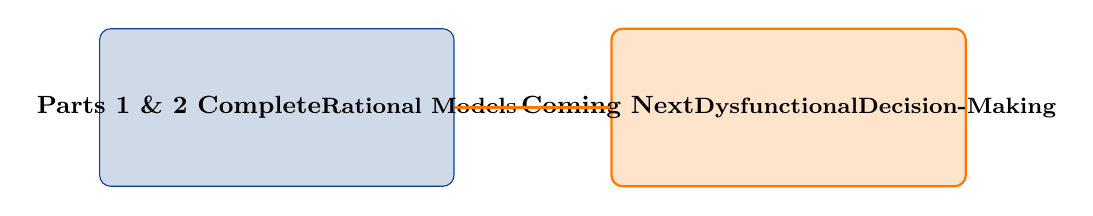
\begin{tikzpicture}[node distance=2cm]
\node[rectangle, rounded corners, minimum width=4.5cm, minimum height=2cm, draw=mediumblue, fill=mediumblue!20] (current) at (0,0) {};
\node[rectangle, rounded corners, minimum width=4.5cm, minimum height=2cm, draw=titanorange, fill=titanorange!20, thick] (part3) at (6.5,0) {};

% Text positioned properly within boxes
\node[font=\small\bfseries] at (current.center) {Parts 1 \& 2 Complete\\[0.2cm]\footnotesize Rational Models};
\node[font=\small\bfseries] at (part3.center) {Coming Next\\[0.2cm]\footnotesize Dysfunctional\\Decision-Making};

\draw[-, thick, titanorange] (current) -- (part3);
\end{tikzpicture}
\end{center}

\vspace{1cm}
\textbf{Next time we'll explore:}
\begin{itemize}
\item Groupthink and its dangers
\item The Garbage Can Model
\item When decision-making goes wrong
\item Safeguards against dysfunction
\end{itemize}
\end{frame}

\end{document}
